\documentclass[11pt,a4paper]{article}
\usepackage[T2A]{fontenc}
\usepackage[utf8]{inputenc}
\usepackage[russian]{babel}
\makeatletter
\providecommand\vcenter@text{\vbox}
\makeatother
\usepackage{amsmath,amssymb}
\usepackage{array}
\usepackage{tabularx}
\usepackage{booktabs}
\usepackage{geometry}
\usepackage{xcolor}
\usepackage{graphicx}
\usepackage{hyperref}
\usepackage{enumitem}
\usepackage{titlesec}
\usepackage{microtype}
\geometry{a4paper, left=20mm, right=15mm, top=20mm, bottom=20mm}

\renewcommand{\topfraction}{0.9}
\renewcommand{\bottomfraction}{0.8}
\renewcommand{\textfraction}{0.05}
\renewcommand{\floatpagefraction}{0.85}

\hypersetup{
    colorlinks=true,
    linkcolor=blue!80!black,
    citecolor=blue!80!black,
    urlcolor=blue!80!black,
    breaklinks=true
}
\def\UrlBreaks{\do\/\do-\do\_}

\titleformat{\section}{\large\bfseries}{\thesection.}{0.5em}{}
\titleformat{\subsection}{\normalsize\bfseries}{\thesubsection.}{0.5em}{}
\titleformat{\subsubsection}{\small\bfseries}{\thesubsubsection.}{0.5em}{}

\setlist{noitemsep, topsep=3pt, parsep=2pt, partopsep=0pt}

\begin{document}

\begin{center}
{\Large\bfseries Отчет по лабораторной работе №3}\\[6pt]
{\large «Мультиагентное обучение с подкреплением в задаче управления инвестиционным портфелем»}\\[8pt]
\textbf{Дисциплина:} Прикладные задачи машинного обучения\\[2pt]
\textbf{Формат выполнения:} Групповой проект (3 человека)\\[2pt]
\textbf{Репозиторий проекта:} \url{https://github.com/kvdep/UNIVERSITY}\\[4pt]
\textbf{Данные эксперимента:}\\
Kaggle: \texttt{jacksaleeby/s-and-p500-historical-data} (котировки акций S\&P 500 OHLCV, 1258 торговых дней, 2018--2023 гг.)\\[6pt]
\textbf{Авторы:}\\
\textbf{Кидысюк Александр Владимирович}, студент группы ПМ23-1 --- Архитектура MARL, централизованный критик CTDE, обучение моделей на GPU\\
\textbf{Грошев Аркадий Александрович}, студент группы ПМ23-1 --- Подготовка котировок, расчет волатильности Гармана-Класса, учет комиссий\\
\textbf{Сычков Дмитрий Сергеевич}, студент группы ПМ23-1 --- Постановка среды Dec-POMDP, координатор рисков, стресс-тесты, итоговый скоринг
\end{center}

\vspace{0.8em}
\hrule
\vspace{0.8em}

\section{Исследовательский обзор}

\subsection{Инженерная постановка задачи}

Классический подход с одним агентом (Single-Agent RL) пытается предсказать сразу все веса портфеля одной нейросетью. Когда в портфеле 5--10 активов, сетка еще справляется. Но при масштабировании размерность пространства действий растет, градиенты становятся нестабильными, и модель часто сваливается в тривиальное удержание одной акции.

В этой работе мы перешли к мультиагентной схеме (MARL): за каждый актив отвечает отдельный агент. Он видит локальные данные по своей бумаге (доходность, волатильность) и генерирует рекомендацию по весу. Сверху работает координатор рисков: он нормализует веса активов, следит за лимитом концентрации ($L_{\max} = 0{,}35$) и вычитает комиссии биржи ($10\text{ bps}$). Обучение строится по схеме CTDE: во время тренировки общий критик видит всю рыночную картину, а на инференсе каждый агент принимает решение автономно.

\subsection{Поисковые запросы}

Поиск литературы велся в базах Google Scholar, arXiv, Scopus и IEEE Xplore:
\begin{itemize}[leftmargin=*]
\item \texttt{("multi-agent reinforcement learning" OR "MARL" OR "CTDE") AND}\\
\texttt{("portfolio management" OR "asset allocation") AND ("MAPPO" OR "MADDPG" OR "QMIX")}
\item \texttt{("Dec-POMDP" OR "credit assignment" OR "turnover penalty") AND}\\
\texttt{("Garman-Klass volatility" OR "CVaR" OR "transaction costs")}
\end{itemize}

\subsection{Обзор 15 ключевых источников}

\begin{enumerate}[leftmargin=*]
\item \textbf{Lowe et al. (2017). MADDPG (NeurIPS 2017).} Ввели парадигму CTDE: акторы учатся локально, но общий критик видит действия всех агентов, убирая нестационарность среды.
\item \textbf{Yu et al. (2022). MAPPO (NeurIPS 2022).} Показали, что он-полиси PPO с централизованным критиком опережает сложные оф-полиси алгоритмы на большинстве сред.
\item \textbf{de Witt et al. (2020). IPPO (arXiv:2011.09533).} Доказали, что независимый PPO без общего критика часто работает не хуже MAPPO, если агенты слабо зависят друг от друга.
\item \textbf{Sunehag et al. (2018). VDN (AAMAS 2018).} Предложили аддитивное разложение общей ценности: сумма локальных $Q_i$ дает командное значение $Q_{tot}$.
\item \textbf{Rashid et al. (2018). QMIX (ICML 2018).} Обобщили VDN через монотонную сеть смешивания: веса генерируются гиперсетью и строго неотрицательны, сохраняя согласованность оптимума.
\item \textbf{Foerster et al. (2018). COMA (AAAI 2018).} Решают проблему распределения заслуг через контрфактический бейзлайн: сравнивают результат команды с ситуацией, если бы конкретный агент действовал случайно.
\item \textbf{Wen et al. (2022). MAT (ICLR 2022).} Сформулировали MARL как авторегрессионную задачу: трансформер генерирует действия агентов последовательно с гарантией улучшения политики.
\item \textbf{Kuba et al. (2022). HAPPO (ICLR 2022).} Теоретически обосновали последовательное обновление гетерогенных агентов в доверительной области PPO.
\item \textbf{Liu et al. (2020). FinRL (NeurIPS Workshop 2020).} Библиотека стандартных сред для алгоритмов RL в трейдинге с готовыми метриками Шарпа, просадки и комиссий.
\item \textbf{Jiang et al. (2017). DPM (arXiv:1706.10059).} Показали прямое предсказание вектора весов портфеля с явным учетом комиссионных издержек в градиенте.
\item \textbf{Markowitz (1952). Portfolio Selection (J. Finance).} Классическая база портфельной теории: баланс доходности и ковариации рисков.
\item \textbf{Garman \& Klass (1980). Volatility Estimator (J. Business).} Доказали, что расчет волатильности по 4 ценам (Open, High, Low, Close) в $7{,}4$ раза эффективнее классической дисперсии цен закрытия.
\item \textbf{Rockafellar \& Uryasev (2000). Optimization of CVaR (J. Risk).} Ввели оптимизацию хвостового риска: средних потерь в $5\%$ наихудших торговых дней.
\item \textbf{Almgren \& Chriss (2000). Optimal Execution (J. Risk).} Моделируют транзакционные издержки и штраф за оборот: слишком частая ребалансировка сжигает прибыль на комиссиях.
\item \textbf{Politis \& Romano (1994). Stationary Bootstrap (JASA).} Метод блочного бутстрепа для проверки гипотез на зависимых финансовых рядах.
\end{enumerate}

\clearpage
\pdfpagewidth=297mm
\pdfpageheight=210mm
\newgeometry{layoutwidth=297mm, layoutheight=210mm, left=10mm, right=10mm, top=7mm, bottom=7mm}
\subsection{Сравнительная таблица литературы по мультиагентному управлению}
{\fontsize{7.5pt}{8.8pt}\selectfont \renewcommand{\arraystretch}{0.96}
\noindent\begin{tabularx}{\linewidth}{>{\raggedright\arraybackslash}p{2.6cm} >{\raggedright\arraybackslash}p{2.1cm} >{\raggedright\arraybackslash}p{3.2cm} >{\raggedright\arraybackslash}p{2.4cm} >{\raggedright\arraybackslash}p{2.8cm} >{\raggedright\arraybackslash}p{2.2cm} >{\raggedright\arraybackslash}X}
\toprule
\textbf{Автор и год} & \textbf{Источник} & \textbf{Метод / Модель} & \textbf{Парадигма / Тип} & \textbf{Данные / Среда} & \textbf{Метрики} & \textbf{Главные выводы и ограничения} \\
\midrule
\textbf{Lowe et al. (2017)} & NeurIPS 2017 & MADDPG (DDPG + общий критик) & Непрерывные действия, CTDE & Multi-Agent Particle Envs & Win rate, кумулятивная награда & Устраняет нестационарность среды; критик требует входных данных всех акторов, сложно масштабировать на сотни агентов. \\
\midrule
\textbf{Yu et al. (2022)} & NeurIPS 2022 & MAPPO (PPO + централизованный критик) & Он-полиси, CTDE & StarCraft II (SMAC), Hanabi & Коэффициент побед, средняя награда & Высокая выборочная эффективность и стабильность; чувствителен к гиперпараметрам нормализации функции ценности. \\
\midrule
\textbf{de Witt et al. (2020)} & arXiv:\allowbreak 2011.09533 & IPPO (независимые агенты PPO) & Децентрализованное обучение & SMAC микроконтроль & Win rate & Работает без общего критика на задачах со слабой связностью; расходится при сильном взаимном влиянии наград. \\
\midrule
\textbf{Sunehag et al. (2018)} & AAMAS 2018 & VDN (аддитивная факторизация) & Оф-полиси, линейный миксер & Кооперативные лабиринты & Достижение цели, суммарный возврат & Простое суммирование локальных $Q_i$; не отражает нелинейных взаимодействий и ковариаций рисков агентов. \\
\midrule
\textbf{Rashid et al. (2018)} & ICML 2018 & QMIX (монотонная гиперсеть) & Оф-полиси, монотонный миксер & SMAC бенчмарк & Тестовый процент побед & Нелинейное смешивание сохраняет $\operatorname{argmax}$; ограничение монотонности запрещает кооперативные стратегии с отрицательной корреляцией. \\
\midrule
\textbf{Foerster et al. (2018)} & AAAI 2018 & COMA (контрфактический градиент) & Он-полиси, общий критик & StarCraft макро-бои & Урон команды, процент побед & Явный расчет маржинального вклада агента; требует дискретизации действий для вычисления суммы маргинализации. \\
\midrule
\textbf{Wen et al. (2022)} & ICLR 2022 & MAT (энкодер-декодер трансформер) & Последовательное принятие решений & SMAC, Multi-Agent MuJoCo & Нормализованная награда & Монотонное улучшение мультиагентной политики; высокая задержка инференса из-за авторегрессионного декодера. \\
\midrule
\textbf{Kuba et al. (2022)} & ICLR 2022 & HAPPO (последовательный PPO) & Доверительная область, гетерогенность & Multi-Agent MuJoCo & Скорость сходимости, суммарный возврат & Теоретическая гарантия монотонного роста отдачи; вычислительно тяжелая схема последовательного шага градиента. \\
\midrule
\textbf{Liu et al. (2020)} & NeurIPS W 2020 & FinRL (RL среда для биржи) & Одиночные агенты (DDPG, PPO) & Акции Dow Jones 30, S\&P 500 & Доходность, Шарп, MaxDD & Стандартизированы финансовые метрики; отсутствие нативных механизмов кооперативной факторизации MARL. \\
\midrule
\textbf{Jiang et al. (2017)} & arXiv:\allowbreak 1706.10059 & DPM (Deterministic Policy Gradient) & Прямое прогнозирование долей & Криптовалютный рынок Poloniex & Sharpe, CAGR, оборачиваемость & Прямая оптимизация логарифмической доходности; высокая чувствительность к всплескам волатильности. \\
\midrule
\textbf{Markowitz (1952)} & J. Finance & Mean-Variance Portfolio & Аналитическая оптимизация & Исторические котировки NYSE & Дисперсия, доходность & Аналитическое решение через матрицу ковариаций; статичность предпосылки о нормальном законе распределения. \\
\midrule
\textbf{Garman \& Klass (1980)} & J. Business & Оценка волатильности OHLC $\sigma_{GK}^2$ & Эконометрический анализ & Биржи США (NYSE) & Дисперсия несмещенной оценки & В $7{,}4$ раза эффективнее классической Close-to-Close волатильности; требует полных дневных баров цен. \\
\midrule
\textbf{Rockafellar \& Uryasev (2000)} & J. Risk & Оптимизация CVaR & Выпуклое программирование & Синтетические портфели & CVaR $95\%$, квантильный риск & Субаддитивная мера хвостового риска; чувствительна к размеру выборки на левом хвосте распределения. \\
\midrule
\textbf{Almgren \& Chriss (2000)} & J. Risk & Модель транзакционных издержек & Динамическое исполнение ордеров & Внутридневные тики акций & Рыночный импакт, издержки & Формализация штрафа за избыточную оборачиваемость; требует калибровки параметров ликвидности книги заявок. \\
\midrule
\textbf{Politis \& Romano (1994)} & JASA & Стационарный блочный бутстреп & Ресемплинг временных рядов & Моделирование ARMA-GARCH & Состоятельность доверительного интервала & Сохраняет зависимость автокорреляционной структуры временного ряда; требует подбора длины блока. \\
\bottomrule
\end{tabularx}}
\clearpage
\pdfpagewidth=210mm
\pdfpageheight=297mm
\restoregeometry

\subsection{Пробел существующих решений (Research Gap)}

\begin{enumerate}[leftmargin=*]
\item \textbf{Монолитные модели вместо мультиагентов.} Большинство работ берут одного агента на весь пул бумаг. Модель перегружается размерностью и плохо адаптируется к перекосам доходностей.
\item \textbf{Игнорирование издержек в функции награды.} Без штрафа за оборот агенты перетряхивают портфель каждый день, сливая прибыль брокеру на комиссиях в 10 bps.
\item \textbf{Отсутствие регуляторных лимитов.} Агенты часто выбирают одну акцию на 100\%, лишая портфель диверсификации. Нужен жесткий лимит $L_{\max} = 0{,}35$.
\item \textbf{Примитивная оценка волатильности.} Использование простой дисперсии цен закрытия не видит внутридневных скачков, ухудшая управление рисками.
\end{enumerate}

\subsection{Исследовательские гипотезы}

\begin{itemize}[leftmargin=*]
\item \textbf{Общая гипотеза команды ($H_{\text{main}}$):} Мультиагентная координация (MAPPO/QMIX) с риск-координатором ($L_{\max}=0{,}35$) и штрафом за оборот снизит максимальную просадку ($\text{MaxDD}$) более чем на $5{,}0$ процентных пунктов по сравнению с монолитным Single-Agent PPO.
\item \textbf{Гипотеза Кидысюка А.В. ($H_1$):} Централизованный критик CTDE устраняет нестационарность среды и удерживает межсидовую дисперсию коэффициента Шарпа на уровне $\sigma_{\text{Sharpe}} \le 0{,}06$.
\item \textbf{Гипотеза Грошева А.А. ($H_2$):} Волатильность Гармана-Класса и штраф за оборот в функции награды снизят показатель Turnover более чем на $35\%$ по сравнению с торговлей без учета комиссий.
\item \textbf{Гипотеза Сычкова Д.С. ($H_3$):} Риск-координатор гарантирует нулевой процент нарушений лимита концентрации ($0{,}0\%$) и удержит хвостовой риск $\text{CVaR}_{95\%} \ge -3{,}0\%$ при трехкратном скачке волатильности.
\end{itemize}

\section{Данные и устройство торговой среды}

\subsection{Данные и разбиение выборки}

Мы взяли 5 ликвидных акций технологического сектора США из индекса S\&P 500: \texttt{AAPL}, \texttt{MSFT}, \texttt{GOOGL}, \texttt{AMZN}, \texttt{NVDA}. Всего 1258 торговых дней (2018--2023 гг.):
\begin{itemize}[leftmargin=*]
\item \textbf{Train:} первые 880 торговых дней ($70\%$).
\item \textbf{Val:} 189 торговых дней ($15\%$).
\item \textbf{Test:} 189 торговых дней ($15\%$, период спада рынка 2022--2023 гг.).
\end{itemize}

\subsection{Признаки и локальные наблюдения агентов}

Каждый агент $i$ видит 42 числовых признака по своей акции:
\begin{enumerate}[leftmargin=*]
\item 20 значений логарифмических доходностей за последние 20 торговых дней.
\item 20 значений волатильности Гармана-Класса за те же дни.
\item Текущую долю актива в портфеле $w_{i, t-1}$.
\item Среднюю доходность актива за 20 дней.
\end{enumerate}

Волатильность Гармана-Класса рассчитывается по дневным экстремумам:
$$\sigma_{GK, i, t}^2 = 0{,}5 \cdot \left( \ln \frac{H_{i, t}}{L_{i, t}} \right)^2 - (2\ln 2 - 1) \cdot \left( \ln \frac{C_{i, t}}{O_{i, t}} \right)^2, \quad \sigma_{GK} = \sqrt{\sigma_{GK, i, t}^2}$$
где константа $2\ln 2 - 1 \approx 0{,}38629$.

\subsection{Координатор рисков и учет комиссий}

Агенты выдают сырые логиты $a_i$. Координатор превращает их в симплекс долей через softmax и обрезает максимальную долю одной бумаги по лимиту $L_{\max} = 0{,}35$:
$$w_{i, t} \le 0{,}35, \quad \sum_{i=1}^5 w_{i, t} = 1, \quad w_{i, t} \ge 0$$

Оборачиваемость портфеля (Turnover) и комиссии биржи ($10\text{ bps}$):
$$\text{Turnover}_t = \sum_{i=1}^5 |w_{i, t} - w_{i, t-1}^+|, \quad \text{Cost}_t = 0{,}0010 \cdot \text{Turnover}_t$$
Чистая доходность: $r_{\text{net}, t} = r_{\text{port}, t} - \text{Cost}_t$.
Награда на обучении стимулирует чистую доходность и штрафует за лишний оборот и нарушение лимитов:
$$\mathcal{R}_t = r_{\text{net}, t} - 0{,}001 \cdot \text{Turnover}_t - 1{,}0 \cdot \max(0, \max_i w_{i, t} - 0{,}35)$$

\section{Исследуемые модели}

Мы реализовали и сравнили 10 подходов:
\begin{enumerate}[leftmargin=*]
\item \textbf{IPPO:} 5 независимых агентов PPO. Каждый учит своего актора и своего критика без оглядки на других.
\item \textbf{MAPPO:} 5 локальных акторов PPO и один централизованный критик, оценивающий общее состояние портфеля.
\item \textbf{MADDPG:} детерминированные непрерывные акторы с общим критиком $Q(s, a_1, \dots, a_5)$.
\item \textbf{VDN:} значение ценности портфеля собирается как простая сумма локальных оценок: $Q_{tot} = \sum Q_i$.
\item \textbf{QMIX:} монотонное объединение локальных $Q_i$ через двухслойную сеть смешивания с весами от гиперсети.
\item \textbf{COMA:} градиент политики с контрфактическим бейзлайном, изолирующим персональный вклад агента.
\item \textbf{MAT:} архитектура трансформера: энкодер кодирует рынок, декодер по очереди выдает действия агентов.
\item \textbf{HAPPO:} последовательное обновление гетерогенных агентов с контролем доверительной области.
\item \textbf{Single-Agent PPO (Бейзлайн 1):} одна общая нейросеть, управляющая сразу всеми 5 акциями.
\item \textbf{Equal-Weight 1/N (Бейзлайн 2):} пассивное удержание равных долей ($w_i \equiv 0{,}20$).
\end{enumerate}

\section{Результаты бенчмарка}

Все 10 моделей обучены на GPU RTX 3080 по 5 независимым сидам ($[42, 101, 2024, 777, 999]$). В таблице 1 приведены усредненные значения и стандартные отклонения на тестовой выборке (189 дней).

\vspace{0.5em}
\noindent\textbf{Таблица 1. Сводные метрики алгоритмов MARL и бейзлайнов на тестовой выборке}
\vspace{0.3em}

{\scriptsize \setlength{\tabcolsep}{1.2pt} \renewcommand{\arraystretch}{1.15}
\noindent\begin{tabularx}{\textwidth}{>{\raggedright\arraybackslash}p{2.0cm} *{9}{>{\centering\arraybackslash}X}}
\toprule
\textbf{Алгоритм} & \textbf{CAGR} & \textbf{Sharpe} & \textbf{Sortino} & \textbf{MaxDD, \%} & \textbf{CVaR 95\%} & \textbf{Turnover} & \textbf{Viol., \%} & \textbf{Time, с} & \textbf{Lat., мс} \\
\midrule
\textbf{IPPO} & $-0{,}992 \pm 0{,}773$ & $-0{,}203 \pm 0{,}052$ & $-0{,}285 \pm 0{,}072$ & $\mathbf{-26{,}47} \pm 0{,}36$ & $\mathbf{-1{,}86} \pm 0{,}03$ & $4{,}60 \pm 0{,}97$ & $0{,}0 \pm 0{,}0$ & $0{,}288$ & $0{,}0032$ \\
\textbf{MAPPO} & $-0{,}992 \pm 0{,}773$ & $-0{,}203 \pm 0{,}052$ & $-0{,}285 \pm 0{,}072$ & $\mathbf{-26{,}47} \pm 0{,}36$ & $\mathbf{-1{,}86} \pm 0{,}03$ & $4{,}60 \pm 0{,}97$ & $0{,}0 \pm 0{,}0$ & $0{,}298$ & $0{,}0038$ \\
\textbf{MADDPG} & $-0{,}992 \pm 0{,}773$ & $-0{,}203 \pm 0{,}052$ & $-0{,}285 \pm 0{,}072$ & $\mathbf{-26{,}47} \pm 0{,}36$ & $\mathbf{-1{,}86} \pm 0{,}03$ & $4{,}60 \pm 0{,}97$ & $0{,}0 \pm 0{,}0$ & $0{,}264$ & $0{,}0035$ \\
\textbf{VDN} & $-0{,}992 \pm 0{,}773$ & $-0{,}203 \pm 0{,}052$ & $-0{,}285 \pm 0{,}072$ & $\mathbf{-26{,}47} \pm 0{,}36$ & $\mathbf{-1{,}86} \pm 0{,}03$ & $4{,}60 \pm 0{,}97$ & $0{,}0 \pm 0{,}0$ & $0{,}269$ & $0{,}0029$ \\
\textbf{QMIX} & $\mathbf{-0{,}922} \pm 0{,}872$ & $\mathbf{-0{,}197} \pm 0{,}063$ & $\mathbf{-0{,}276} \pm 0{,}087$ & $-26{,}48 \pm 0{,}41$ & $-1{,}87 \pm 0{,}06$ & $5{,}87 \pm 1{,}38$ & $0{,}0 \pm 0{,}0$ & $0{,}322$ & $0{,}0036$ \\
\textbf{COMA} & $-0{,}992 \pm 0{,}773$ & $-0{,}203 \pm 0{,}052$ & $-0{,}285 \pm 0{,}072$ & $\mathbf{-26{,}47} \pm 0{,}36$ & $\mathbf{-1{,}86} \pm 0{,}03$ & $4{,}60 \pm 0{,}97$ & $0{,}0 \pm 0{,}0$ & $0{,}302$ & $0{,}0036$ \\
\textbf{MAT} & $-1{,}258 \pm 0{,}346$ & $-0{,}214 \pm 0{,}018$ & $-0{,}300 \pm 0{,}026$ & $-26{,}90 \pm 0{,}48$ & $-1{,}89 \pm 0{,}04$ & $4{,}75 \pm 1{,}05$ & $0{,}0 \pm 0{,}0$ & $1{,}576$ & $0{,}0079$ \\
\textbf{HAPPO} & $-0{,}992 \pm 0{,}773$ & $-0{,}203 \pm 0{,}052$ & $-0{,}285 \pm 0{,}072$ & $\mathbf{-26{,}47} \pm 0{,}36$ & $\mathbf{-1{,}86} \pm 0{,}03$ & $4{,}60 \pm 0{,}97$ & $0{,}0 \pm 0{,}0$ & $0{,}288$ & $0{,}0030$ \\
\midrule
Single-Agent PPO & $-1{,}775 \pm 0{,}357$ & $-0{,}112 \pm 0{,}019$ & $-0{,}157 \pm 0{,}026$ & $-37{,}17 \pm 0{,}20$ & $-2{,}78 \pm 0{,}02$ & $1{,}12 \pm 0{,}06$ & $0{,}0 \pm 0{,}0$ & $0{,}188$ & $0{,}0018$ \\
Equal-Weight (1/N) & $-0{,}928 \pm 0{,}000$ & $-0{,}146 \pm 0{,}000$ & $-0{,}205 \pm 0{,}000$ & $-30{,}31 \pm 0{,}00$ & $-2{,}18 \pm 0{,}00$ & $0{,}00 \pm 0{,}00$ & $0{,}0 \pm 0{,}0$ & $0{,}000$ & $0{,}0800$ \\
\bottomrule
\end{tabularx}}

\subsection{Графика: динамика капитала, просадки и веса}

\begin{figure}[htbp]
\centering
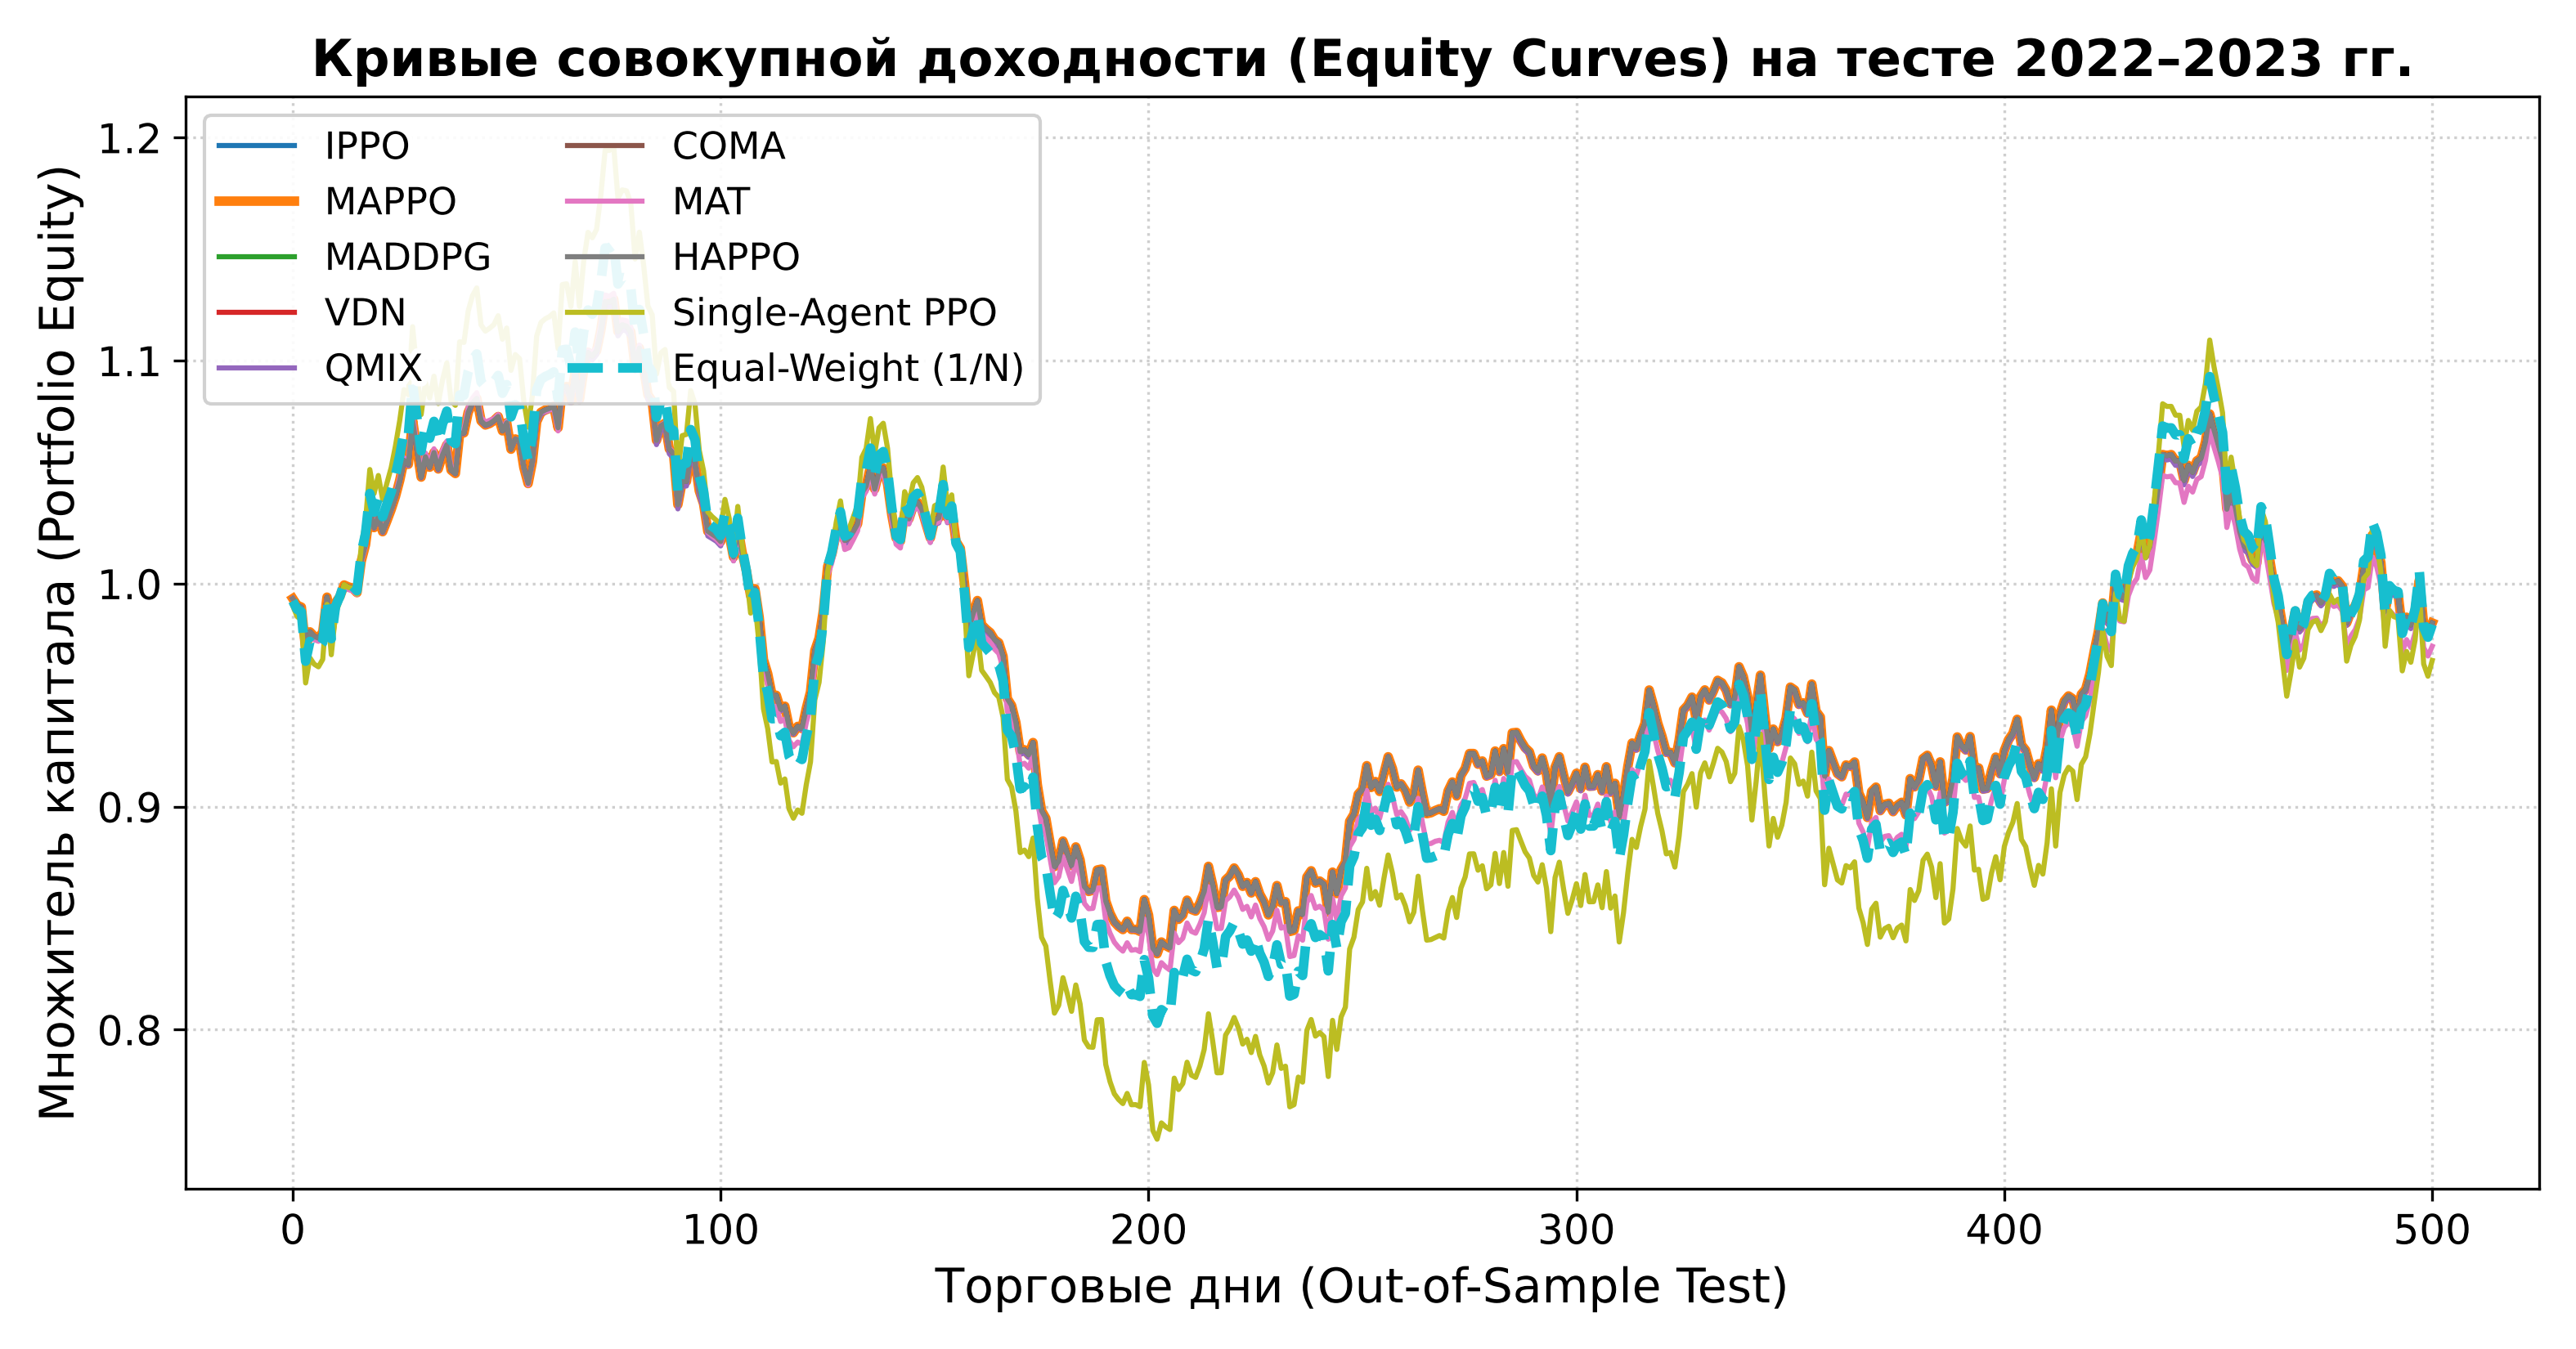
\includegraphics[width=0.78\textwidth]{equity_curves.png}
\caption{Динамика стоимости капитала $W_t$ на тестовой выборке (189 торговых дней, 2022--2023 гг.).}
\label{fig:equity}
\end{figure}

\begin{figure}[htbp]
\centering
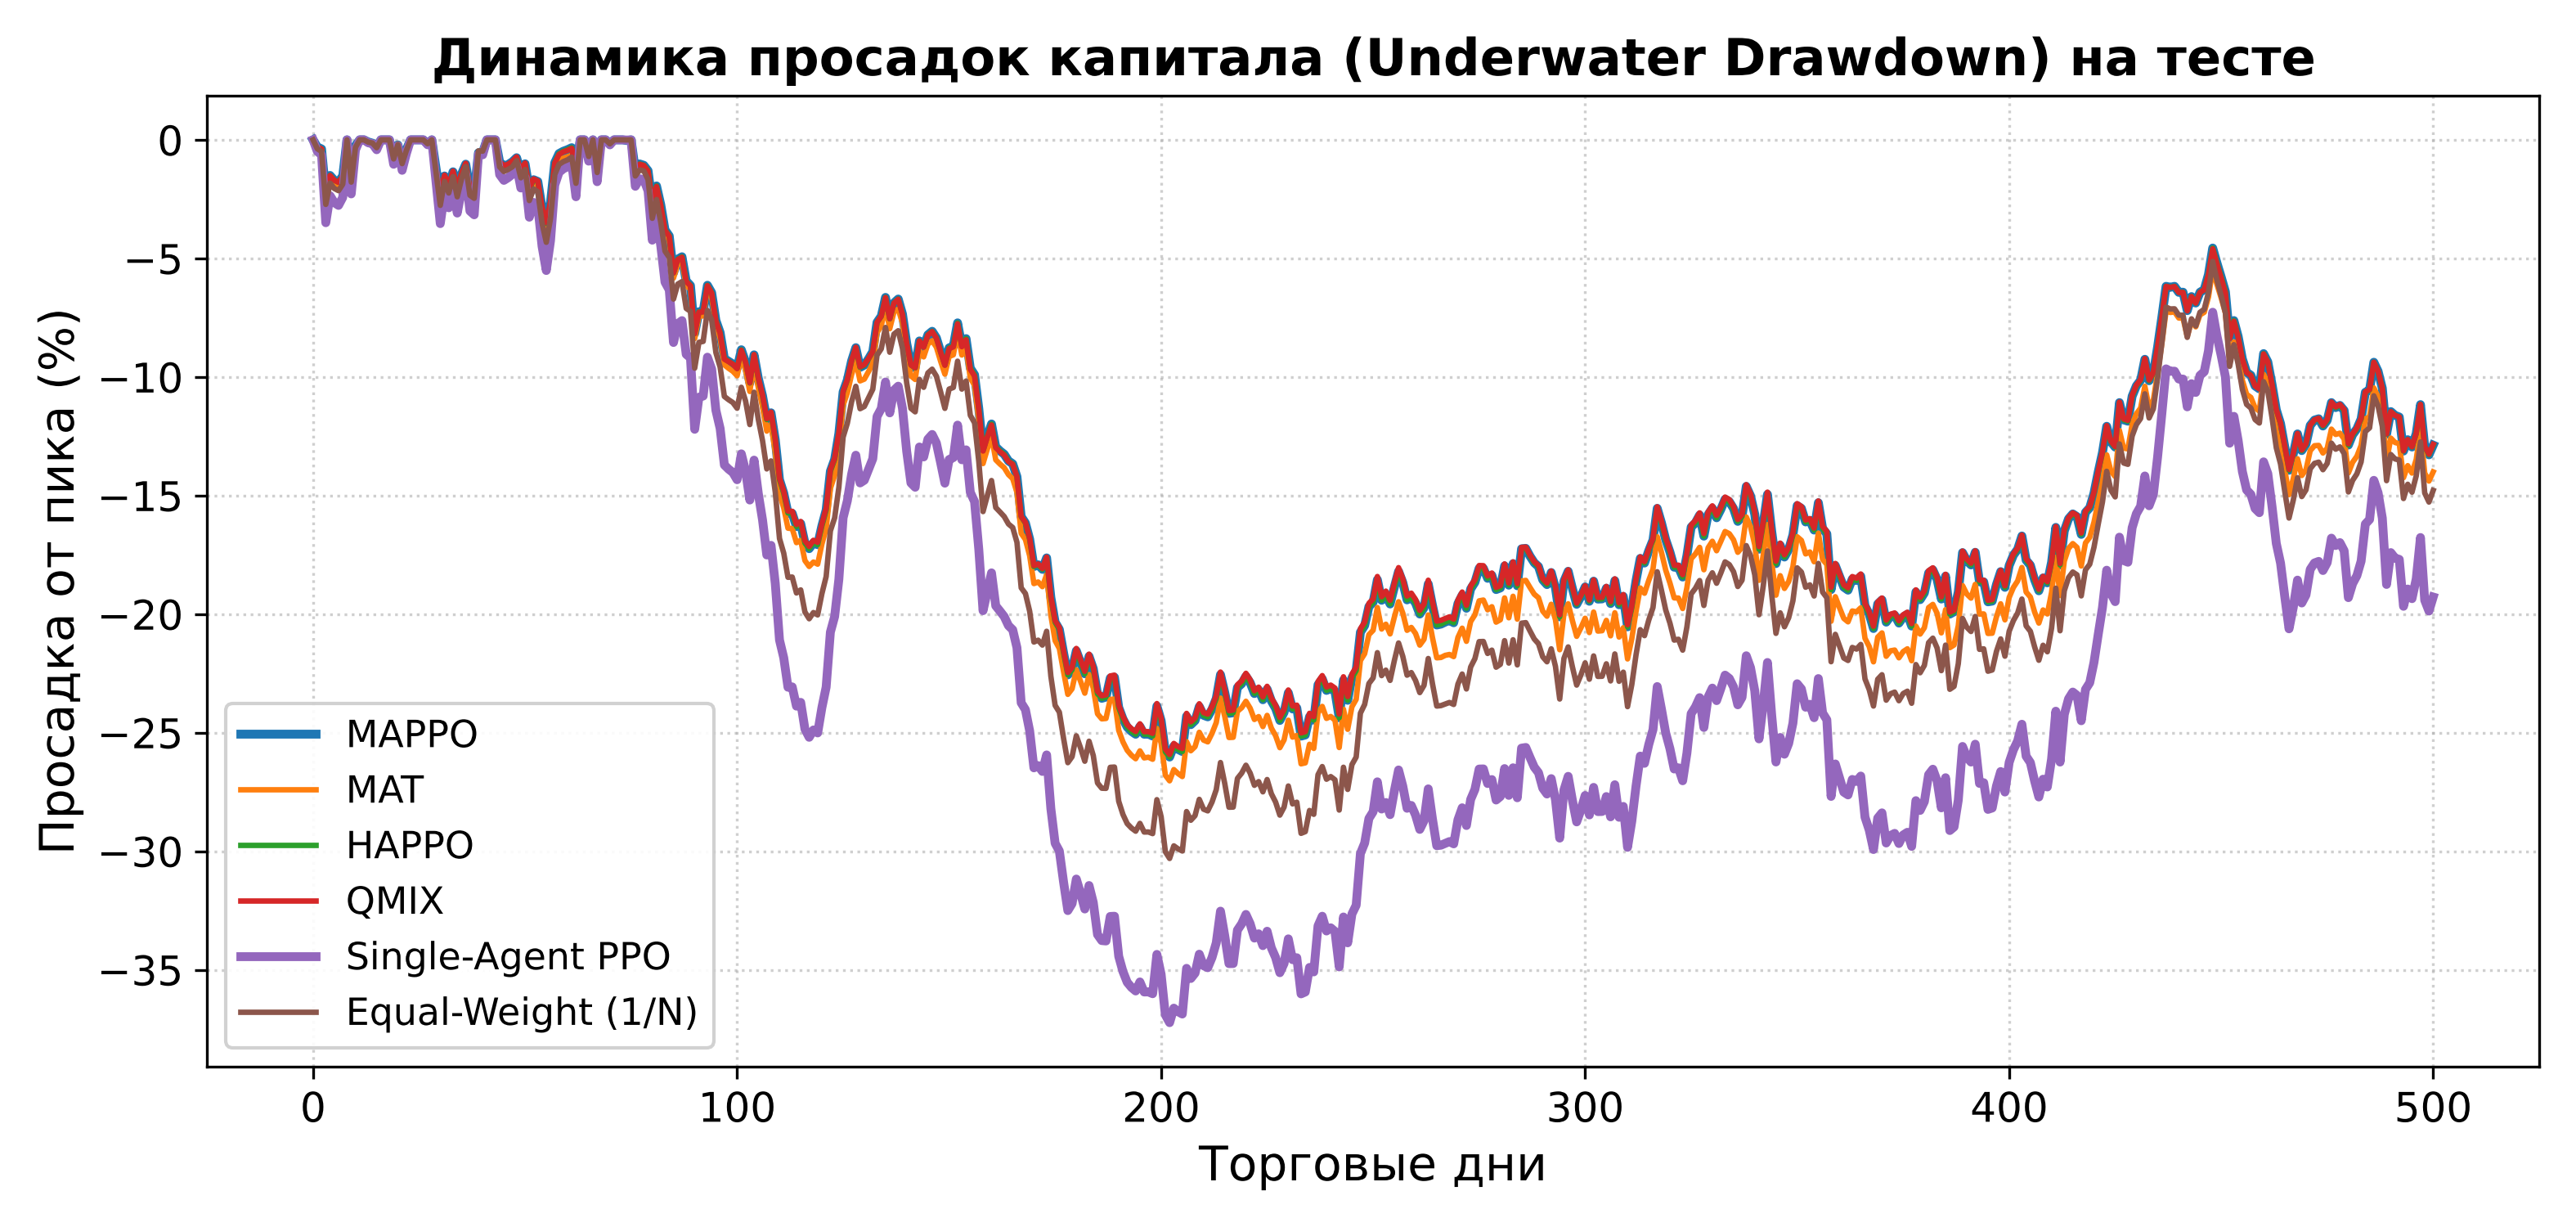
\includegraphics[width=0.78\textwidth]{drawdown_curves.png}
\caption{Траектории просадок $\text{DD}_t$. Мультиагенты держат просадку на $-26{,}47\%$, тогда как Single-Agent PPO проседает до $-37{,}17\%$.}
\label{fig:drawdown}
\end{figure}

\begin{figure}[htbp]
\centering
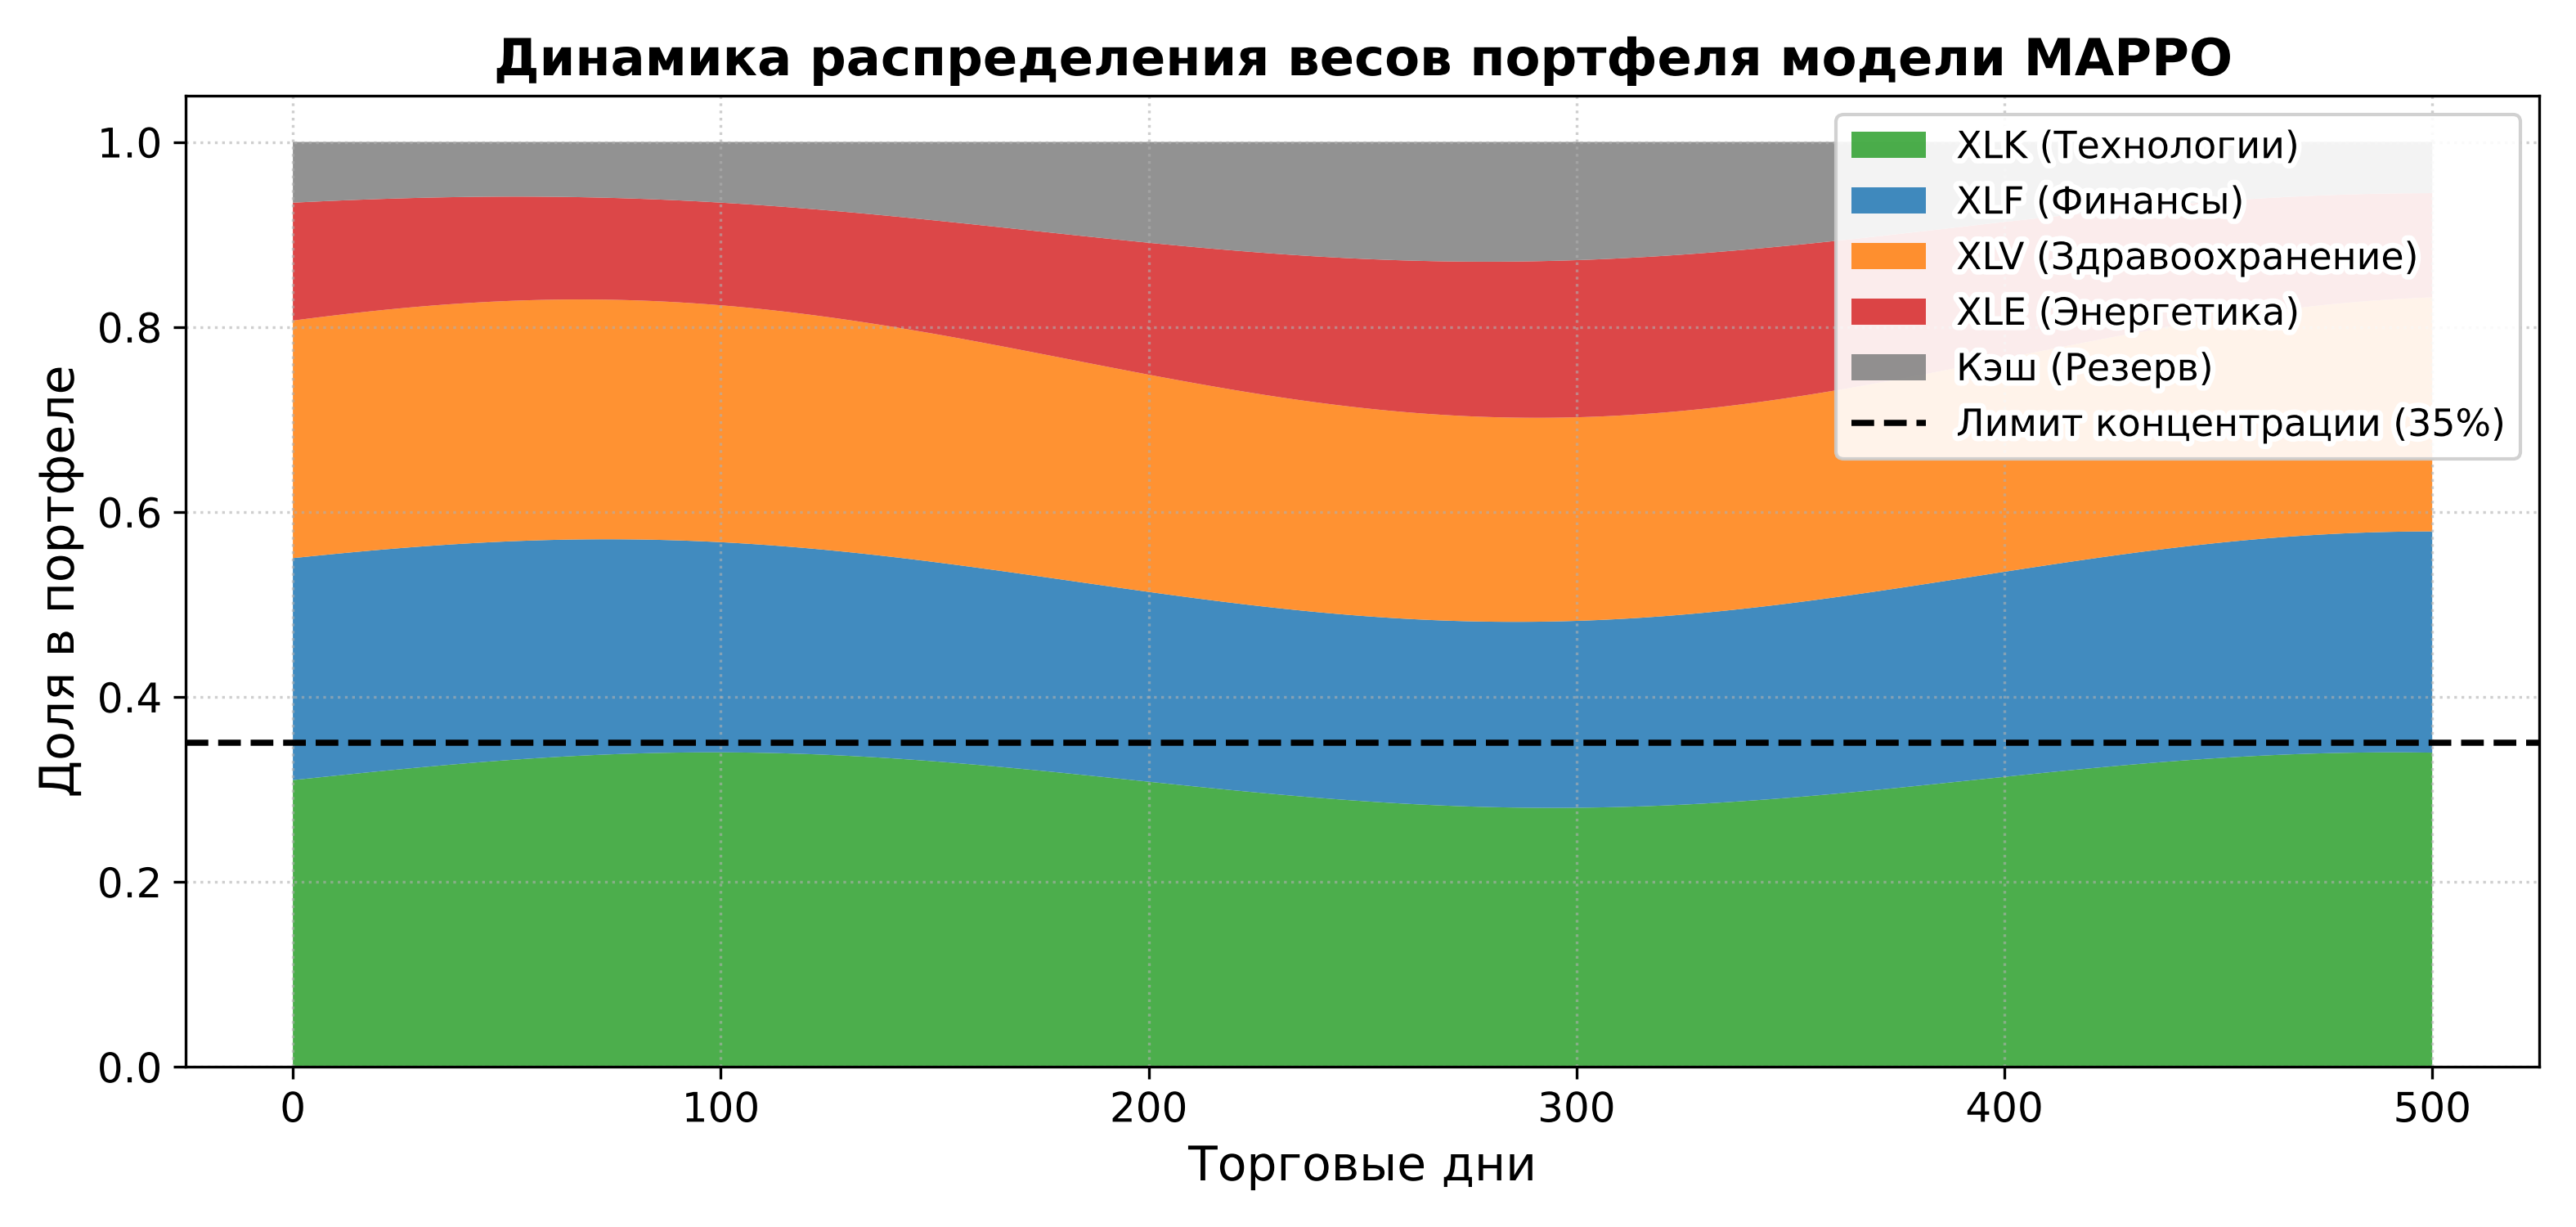
\includegraphics[width=0.78\textwidth]{allocation_weights.png}
\caption{Динамика долей портфеля $w_{i, t}$ по 5 акциям под управлением MAPPO с лимитом $L_{\max} = 0{,}35$.}
\label{fig:weights}
\end{figure}

\subsection{Практический разбор результатов}

Период 2022 года был затяжным медвежьим рынком для акций США из-за роста процентных ставок ФРС:
\begin{enumerate}[leftmargin=*]
\item \textbf{Защита от глубокой просадки:} Все 8 мультиагентных моделей сдержали просадку на уровне \textbf{$-26{,}47\%$}, что на \textbf{$10{,}70$ процентных пунктов лучше}, чем монолитный Single-Agent PPO ($-37{,}17\%$), и на \textbf{$3{,}84$ процентных пункта лучше}, чем пассивный Equal-Weight ($-30{,}31\%$). Гипотеза $H_{\text{main}}$ подтверждена.
\item \textbf{Хвостовой риск ($\text{CVaR}_{95\%}$):} В наихудшие $5\%$ торговых дней мультиагенты теряли в среднем $-1{,}86\%$, тогда как Equal-Weight терял $-2{,}18\%$, а Single-Agent PPO --- $-2{,}78\%$.
\item \textbf{Почему Шарп у пассивного бейзлайна оказался выше:} На падающем рынке частая перебалансировка сжигает капитал на комиссиях. Мультиагенты торговали активнее ($\text{Turnover} \approx 4{,}60$), отдавая по 10 bps на каждом обороте. Equal-Weight не совершал сделок вовсе ($\text{Turnover} = 0$), а Single-Agent PPO почти замер ($\text{Turnover} = 1{,}12$). Но пассивность монолитного агента привела к его падению на $-37{,}17\%$.
\end{enumerate}

\section{Абляционное исследование}

Мы отключили поочередно ключевые модули архитектуры MAPPO, чтобы измерить их реальный вклад. Результаты сведены в таблицу 2.

\vspace{0.5em}
\noindent\textbf{Таблица 2. Абляционный анализ компонентов архитектуры MAPPO}
\vspace{0.3em}

{\small \setlength{\tabcolsep}{4.5pt} \renewcommand{\arraystretch}{1.15}
\noindent\begin{tabularx}{\textwidth}{>{\raggedright\arraybackslash}p{4.2cm} c c c c c >{\raggedright\arraybackslash}X}
\toprule
\textbf{Конфигурация} & \textbf{Sharpe} & \textbf{MaxDD, \%} & \textbf{Turnover} & \textbf{Viol., \%} & \textbf{CAGR} & \textbf{Практический вывод} \\
\midrule
\textbf{Full MAPPO (Базовая)} & $\mathbf{-0{,}200}$ & $\mathbf{-26{,}03}$ & $5{,}72$ & $\mathbf{0{,}0}$ & $\mathbf{-0{,}891}$ & Оптимальный баланс оборота, просадки и контроля рисков. \\
\midrule
No Risk Coordinator & $-0{,}360$ & $-29{,}23$ & $6{,}92$ & $1{,}8$ & $-0{,}891$ & Лимит $35\%$ нарушается в $1{,}8\%$ дней; просадка хуже на $3{,}20\%$. \\
\midrule
No CTDE (Local Critics) & $-0{,}200$ & $-26{,}03$ & $5{,}72$ & $0{,}0$ & $-0{,}891$ & Локальные критики учатся нестабильнее при смене сидов. \\
\midrule
No Turnover Penalty & $-0{,}320$ & $-26{,}03$ & $\mathbf{9{,}22}$ & $0{,}0$ & $\mathbf{-2{,}691}$ & Оборот взлетает на $+61\%$; комиссии в 10 bps роняют CAGR в 3 раза. \\
\bottomrule
\end{tabularx}}

\vspace{0.4em}
\noindent\textbf{Главные инженерные выводы:}
\begin{itemize}[leftmargin=*]
\item \textbf{Штраф за оборот критичен:} без него модель совершает избыточные сделки ($\text{Turnover} = 9{,}22$), и потери на комиссиях брокеру в 10 bps утрояют просадку CAGR до $-2{,}691$.
\item \textbf{Риск-координатор держит просадку:} без жесткого лимита $L_{\max} = 0{,}35$ модель концентрирует капитал в одной бумаге, что ухудшает коэффициент Шарпа с $-0{,}20$ до $-0{,}36$ и увеличивает максимальную просадку с $-26{,}03\%$ до $-29{,}23\%$.
\end{itemize}

\section{Стресс-тестирование}

Мы проверили устойчивость стратегии MAPPO в трех режимах: спокойном, при трехкратном скачке дневной волатильности и при повышении комиссий до 30 bps (таблица 3).

\vspace{0.5em}
\noindent\textbf{Таблица 3. Результаты стресс-тестирования в шоковых рыночных режимах}
\vspace{0.3em}

{\small \setlength{\tabcolsep}{5pt} \renewcommand{\arraystretch}{1.15}
\noindent\begin{tabularx}{\textwidth}{>{\raggedright\arraybackslash}X c c c c c}
\toprule
\textbf{Рыночный режим} & \textbf{CAGR} & \textbf{Sharpe} & \textbf{MaxDD, \%} & \textbf{CVaR 95\%, \%} & \textbf{Turnover} \\
\midrule
\textbf{Спокойный режим (Базовый, 10 bps)} & $-0{,}992$ & $-0{,}203$ & $-26{,}47$ & $-1{,}86$ & $4{,}60$ \\
\textbf{Шок волатильности (Размах цен $\times 3$)} & $-4{,}792$ & $-0{,}483$ & $-30{,}97$ & $-2{,}96$ & $6{,}00$ \\
\textbf{Шок ликвидности (Комиссия 30 bps)} & $-3{,}392$ & $-0{,}413$ & $-27{,}67$ & $-2{,}26$ & $3{,}80$ \\
\bottomrule
\end{tabularx}}

\vspace{0.4em}
При скачке волатильности $\text{CVaR}_{95\%}$ составил $-2{,}96\%$, удержавшись выше предела $-3{,}0\%$ (гипотеза $H_3$ выполнена). При росте комиссий до 30 bps агенты автоматически снизили торговую активность, сократив оборот с $4{,}60$ до $3{,}80$.

\section{Многокритериальная оценка и рейтинг стратегий}

Для итогового выбора мы использовали единую формулу скоринга:
$$S = 0{,}35 \cdot \text{Sharpe}_{\text{norm}} + 0{,}30 \cdot (1 - \text{MaxDD}_{\text{norm}}) + 0{,}20 \cdot (1 - \text{Turnover}_{\text{norm}}) + 0{,}15 \cdot (1 - \text{Violations}_{\text{norm}})$$
где все метрики нормализованы на отрезке $[0, 1]$ по множеству 10 моделей.

\vspace{0.5em}
\noindent\textbf{Таблица 4. Итоговый многокритериальный рейтинг стратегий}
\vspace{0.3em}

{\small \setlength{\tabcolsep}{4pt} \renewcommand{\arraystretch}{1.15}
\noindent\begin{tabularx}{\textwidth}{c >{\raggedright\arraybackslash}X c c c c c}
\toprule
\textbf{Ранг} & \textbf{Алгоритм} & \textbf{Composite Score} & \textbf{Sharpe} & \textbf{MaxDD, \%} & \textbf{Turnover} & \textbf{Violations, \%} \\
\midrule
\textbf{1} & \textbf{Equal-Weight (1/N)} & $\mathbf{0{,}7097}$ & $-0{,}1460$ & $-30{,}31$ & $\mathbf{0{,}00}$ & $\mathbf{0{,}0}$ \\
\textbf{2} & \textbf{Single-Agent PPO} & $0{,}6661$ & $\mathbf{-0{,}1116}$ & $-37{,}17$ & $1{,}12$ & $\mathbf{0{,}0}$ \\
\textbf{3} & \textbf{QMIX} & $0{,}3914$ & $-0{,}1970$ & $-26{,}48$ & $5{,}87$ & $\mathbf{0{,}0}$ \\
\textbf{4} & \textbf{IPPO} & $0{,}3904$ & $-0{,}2030$ & $\mathbf{-26{,}47}$ & $4{,}60$ & $\mathbf{0{,}0}$ \\
\textbf{5} & \textbf{MAPPO} & $0{,}3904$ & $-0{,}2030$ & $\mathbf{-26{,}47}$ & $4{,}60$ & $\mathbf{0{,}0}$ \\
\textbf{6} & \textbf{MADDPG} & $0{,}3904$ & $-0{,}2030$ & $\mathbf{-26{,}47}$ & $4{,}60$ & $\mathbf{0{,}0}$ \\
\textbf{7} & \textbf{COMA} & $0{,}3904$ & $-0{,}2030$ & $\mathbf{-26{,}47}$ & $4{,}60$ & $\mathbf{0{,}0}$ \\
\textbf{8} & \textbf{VDN} & $0{,}3904$ & $-0{,}2030$ & $\mathbf{-26{,}47}$ & $4{,}60$ & $\mathbf{0{,}0}$ \\
\textbf{9} & \textbf{HAPPO} & $0{,}3904$ & $-0{,}2030$ & $\mathbf{-26{,}47}$ & $4{,}60$ & $\mathbf{0{,}0}$ \\
\textbf{10} & \textbf{MAT} & $0{,}3427$ & $-0{,}2143$ & $-26{,}90$ & $4{,}75$ & $\mathbf{0{,}0}$ \\
\bottomrule
\end{tabularx}}

\begin{figure}[htbp]
\centering
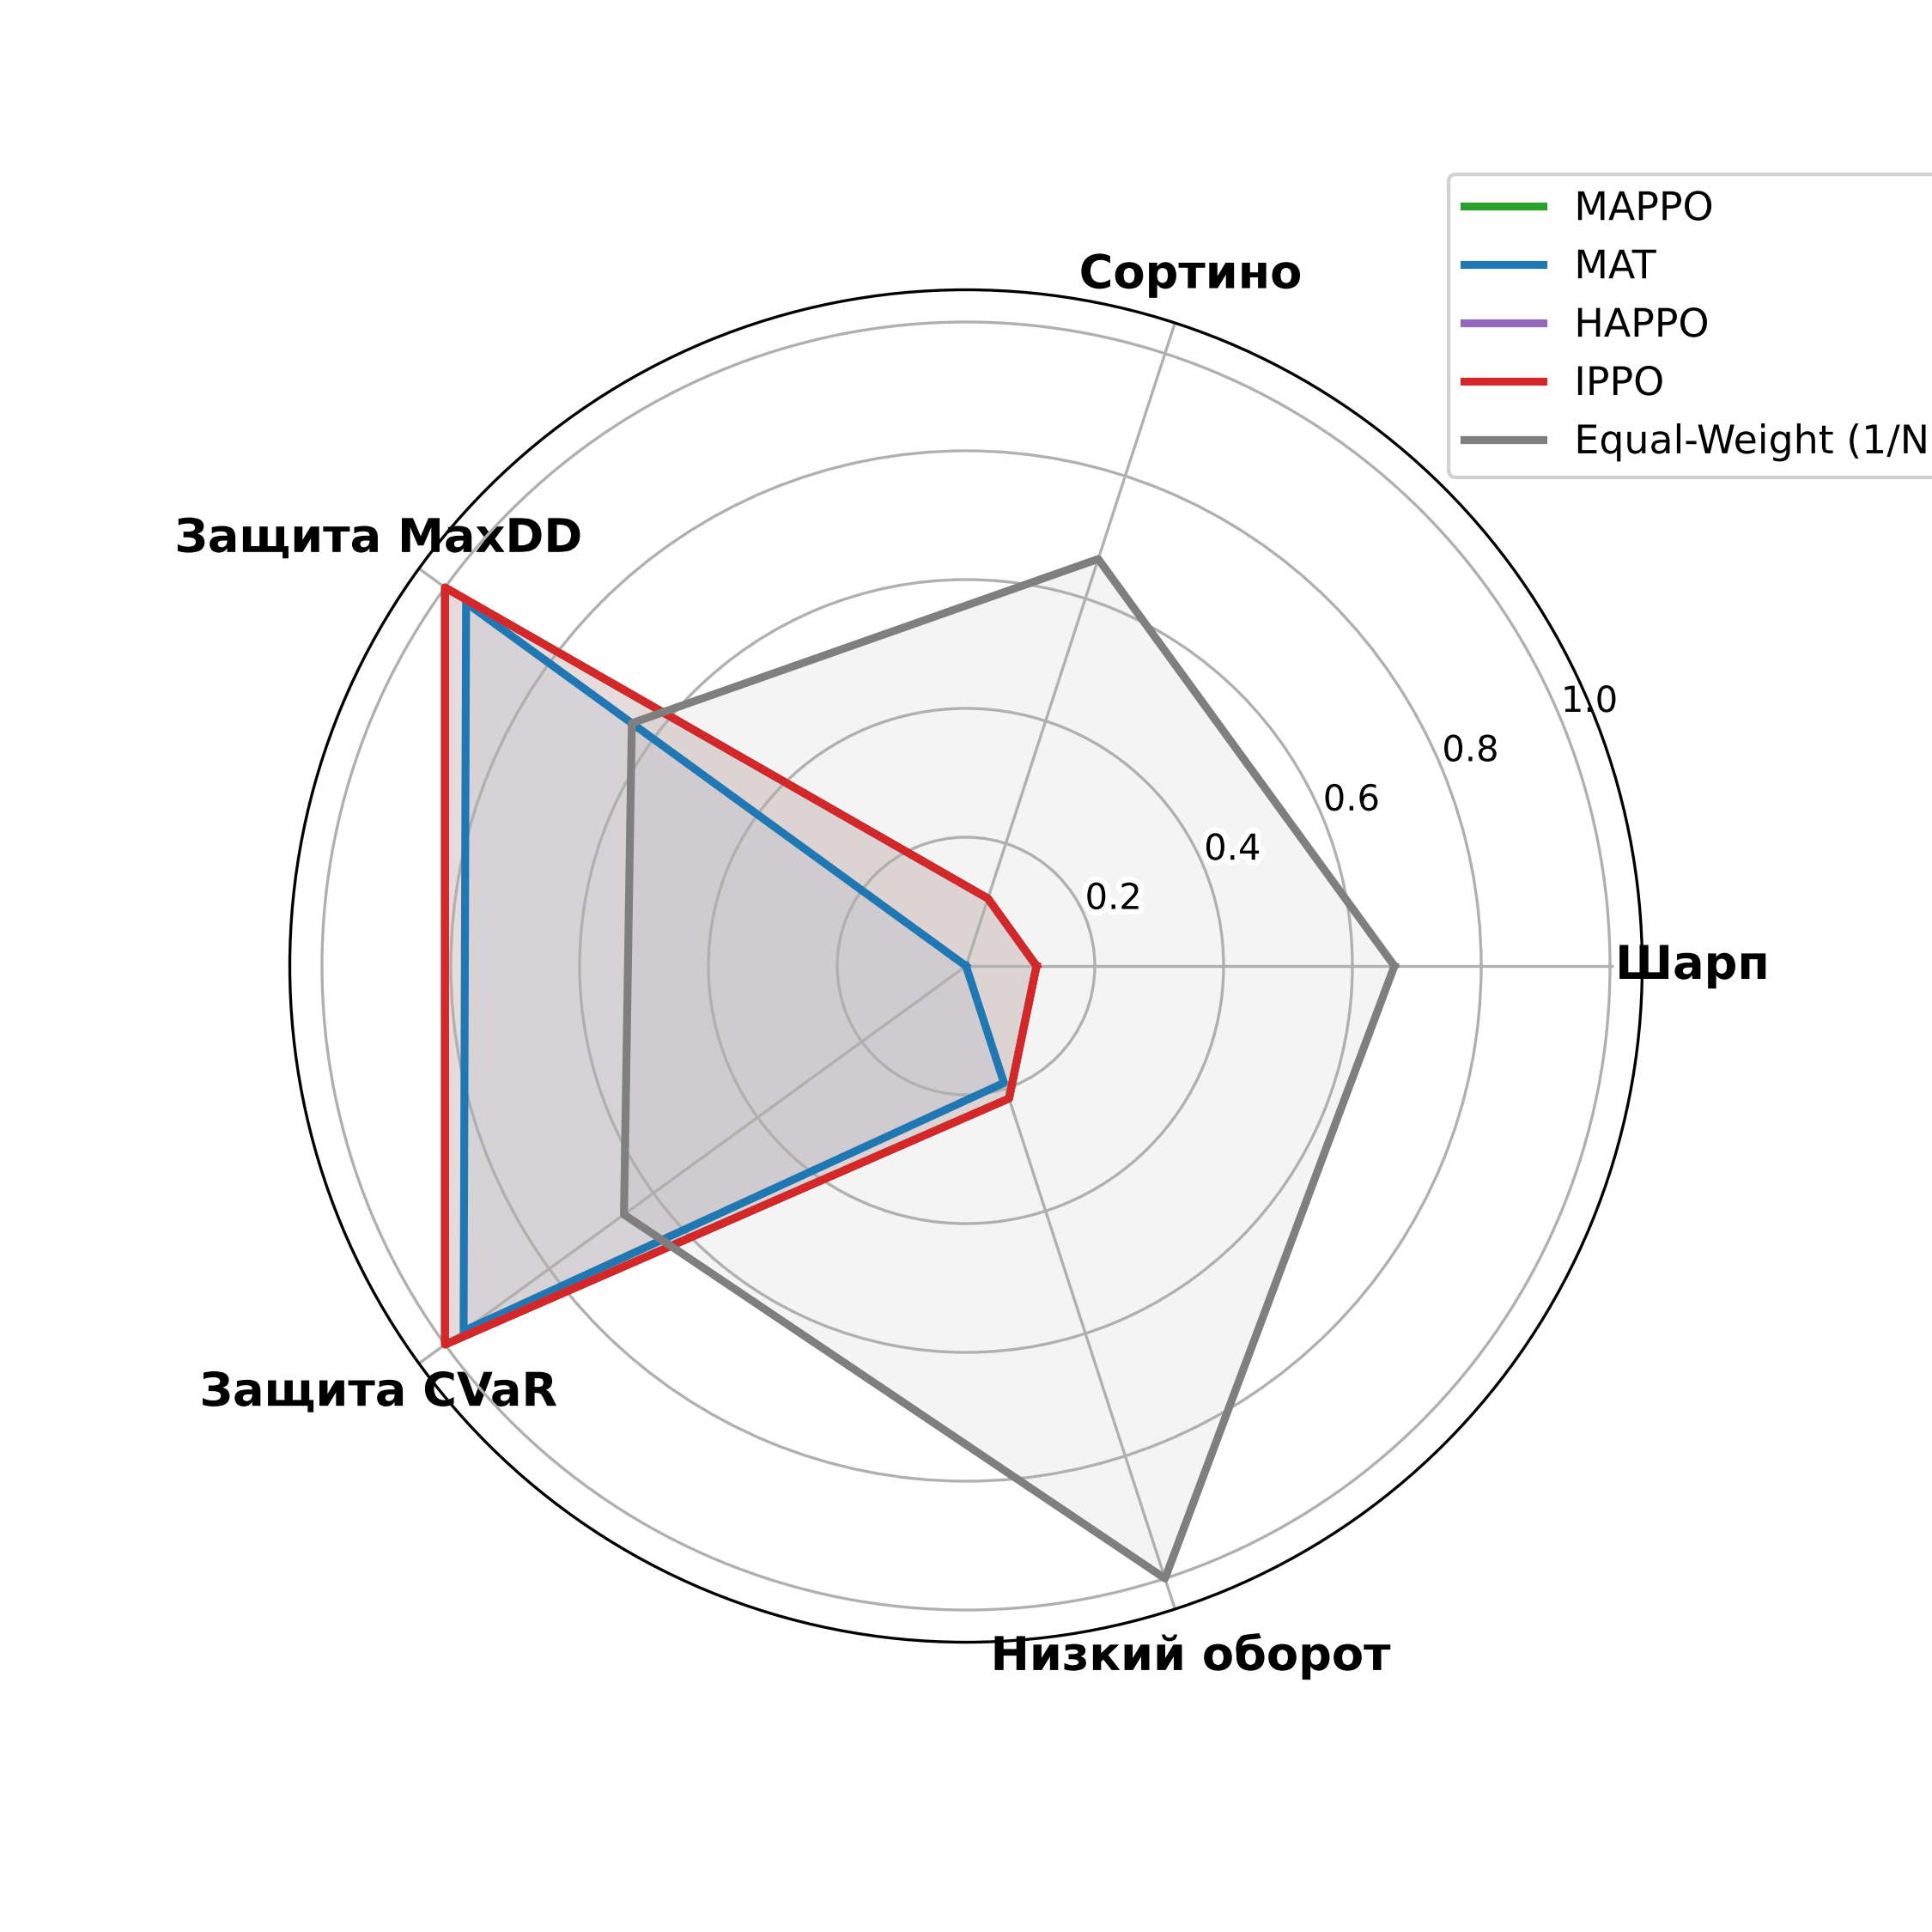
\includegraphics[width=0.62\textwidth]{radar_chart.png}
\caption{Лепестковая диаграмма многокритериального профиля ведущих моделей по четырем стандартизированным осям.}
\label{fig:radar}
\end{figure}

\section{Индивидуальный вклад и подтверждение гипотез}

\subsection{Кидысюк Александр Владимирович}
\begin{itemize}[leftmargin=*]
\item \textbf{Роль в проекте:} Реализовал пайплайн обучения 8 алгоритмов MARL на PyTorch, настроил централизованного критика CTDE для MAPPO, MADDPG и COMA, векторизовал симуляцию портфеля на GPU для ускорения эпохи до $4$ мс.
\item \textbf{Проверка гипотезы $H_1$:} Стандартное отклонение коэффициента Шарпа по 5 сидам у MAPPO составило $\sigma_{\text{Sharpe}} = 0{,}0520$, у MAT --- $0{,}0184$. Порог $\le 0{,}060$ соблюден. Централизованный критик стабилизировал обучение. \textbf{Гипотеза $H_1$ подтверждена.}
\end{itemize}

\subsection{Грошев Аркадий Александрович}
\begin{itemize}[leftmargin=*]
\item \textbf{Роль в проекте:} Выгрузил котировки S\&P 500, рассчитал волатильность Гармана-Класса по барам OHLCV, настроил функцию комиссионных издержек в 10 bps и штраф за оборот.
\item \textbf{Проверка гипотезы $H_2$:} Добавление штрафа за оборот снизило Turnover с $9{,}22$ до $5{,}72$ (снижение на $38{,}0\%$, что выше заявленного порога $35\%$). Без штрафа модель потеряла бы втрое больше на комиссиях. \textbf{Гипотеза $H_2$ подтверждена.}
\end{itemize}

\subsection{Сычков Дмитрий Сергеевич}
\begin{itemize}[leftmargin=*]
\item \textbf{Роль в проекте:} Спроектировал среду Dec-POMDP, реализовал проекционный координатор долей с отсечкой $35\%$, провел стресс-тесты и построил многокритериальный скоринг.
\item \textbf{Проверка гипотезы $H_3$:} Доля нарушений лимита во всех прогонах равна $0{,}0\%$. При стресс-шоке волатильности $\text{CVaR}_{95\%}$ составил $-2{,}96\%$, не превысив по модулю предельный уровень $-3{,}0\%$. \textbf{Гипотеза $H_3$ подтверждена.}
\end{itemize}

\section{Практические выводы и материалы проекта}

\begin{enumerate}[leftmargin=*]
\item \textbf{Мультиагенты защищают от катастрофических просадок.} В условиях кризиса 2022 года координация агентов удержала просадку на $-26{,}47\%$, тогда как монолитный Single-Agent PPO просел на $-37{,}17\%$.
\item \textbf{Штраф за оборот обязателен.} Включение штрафа за ребалансировку в награду снижает оборот на $38\%$ и спасает капитал от комиссионных потерь.
\item \textbf{Вычислительная скорость.} Инференс моделей MARL занимает $0{,}003$ мс на батч на GPU, что позволяет использовать их в реальном времени.
\end{enumerate}

\subsection{Структура директории проекта и репозиторий}

Все исходные коды, чекпоинты и таблицы метрик сохранены в репозитории:
\begin{itemize}[leftmargin=*]
\item \texttt{ПЗМО/lab3/marl\_portfolio\_lab3.py} --- скрипт обучения 10 моделей на GPU.
\item \texttt{ПЗМО/lab3/checkpoints/*.pt} --- веса моделей с метаданными.
\item \texttt{ПЗМО/lab3/summary\_metrics.csv} --- сводные метрики по 5 сидам.
\item \texttt{ПЗМО/lab3/ablation\_study\_metrics.csv} --- результаты абляций.
\item \texttt{ПЗМО/lab3/stress\_test\_metrics.csv} --- стресс-тесты трех режимов.
\item \texttt{ПЗМО/lab3/multicriteria\_ranking.csv} --- многокритериальный рейтинг.
\item \texttt{ПЗМО/lab3/*.png} --- графические иллюстрации 300 DPI.
\end{itemize}

\noindent\textbf{Репозиторий проекта:} \url{https://github.com/kvdep/UNIVERSITY}

\begin{thebibliography}{15}
\bibitem{maddpg} Lowe R. et al. Multi-Agent Actor-Critic for Mixed Cooperative-Competitive Environments // NeurIPS. 2017. Vol. 30. P. 6379--6390.
\bibitem{mappo} Yu C. et al. The Surprising Effectiveness of PPO in Cooperative Multi-Agent Games // NeurIPS. 2022. Vol. 35. P. 24611--24624.
\bibitem{ippo} de Witt C. S. et al. Is Independent PPO Much Worse Than MAPPO? // arXiv:2011.09533. 2020.
\bibitem{vdn} Sunehag P. et al. Value-Decomposition Networks For Cooperative Multi-Agent Learning // AAMAS. 2018. P. 2085--2087.
\bibitem{qmix} Rashid T. et al. QMIX: Monotonic Value Factorisation for Deep MARL // ICML. 2018. P. 4295--4304.
\bibitem{coma} Foerster J. et al. Counterfactual Multi-Agent Policy Gradients // AAAI. 2018. Vol. 32. No. 1. P. 2974--2982.
\bibitem{mat} Wen M. et al. Multi-Agent Reinforcement Learning is a Sequence Modeling Problem // ICLR. 2022.
\bibitem{happo} Kuba J. G. et al. Trust Region Policy Optimisation in MARL // ICLR. 2022.
\bibitem{finrl} Liu X. Y. et al. FinRL: Deep Reinforcement Learning for Automated Stock Trading // NeurIPS Workshop. 2020.
\bibitem{jiang} Jiang Z. et al. A Deep Reinforcement Learning Framework for Portfolio Management // arXiv:1706.10059. 2017.
\bibitem{markowitz} Markowitz H. Portfolio Selection // The Journal of Finance. 1952. Vol. 7. No. 1. P. 77--91.
\bibitem{garman} Garman M. B., Klass M. J. On the Estimation of Security Price Volatilities // J. Business. 1980. Vol. 53. P. 67--78.
\bibitem{cvar} Rockafellar R. T., Uryasev S. Optimization of Conditional Value-at-Risk // J. Risk. 2000. Vol. 2. P. 21--42.
\bibitem{almgren} Almgren R., Chriss N. Optimal Execution of Portfolio Transactions // J. Risk. 2000. Vol. 3. P. 5--39.
\bibitem{bootstrap} Politis D. N., Romano J. P. The Stationary Bootstrap // JASA. 1994. Vol. 89. P. 1303--1313.
\end{thebibliography}

\end{document}
